\chapter{User Guided Synthesis of an \iic\ Driver}
\label{ch:worked_example}

In this appendix we step through synthesis of the driver for a simple but real device. The device we are targeting is an \iic\ controller on a Samsung Exynos~5 system on ship. We assume the there is no operating system i.e.\ the driver runs on bare metal.

We start with the operating system specification. This gives us the interface that the driver is expected to provide. \iic\ is a bus protocol typically used to attach low speed devices to a processor. \iic\ transactions take place between a master device and a slave device. They are always initiated by the master, which may request a read or a write. Each device on an \iic\ bus has an address which is used by the master to identify the slave that it wants to communicate with. In this walkthrough, we will synthesize the driver code necessary to perform a write in master mode. 

\iic\ transactions occur in three phases:
\begin{enumerate}
    \item The transaction is initiated and the address of the slave that the master wants to communicate with is placed on the bus.
    \item The master sends some number $N$ of bytes.
    \item The master ends the transaction by sending a stop bit.
\end{enumerate}

\section{Driver template}

Our driver interface provides three functions, \code{send\_address()}, \code{send\_data()} and \code{send\_stop()}, one for each phase. In C code, the driver may be used like so:
\begin{figure}
\caption{Usage of the \iic driver}
\label{fig:iic_usage}
\begin{lstlisting}[frame=single]
send_address(0xAD);

//Call the below function as many times as you like:
send_data(dat0);
send_data(dat1);
send_data(dat2);

send_stop();
\end{lstlisting}
\end{figure}

Additionally, it provides a function called \code{configure()} that initialises the device so that it is ready to perform transactions.

We declare these required functions in the driver template:
\vspace*{5mm}
\lstinputlisting[style=tsl2]{i2c/drv.tsl}
\vspace*{5mm}

Each function stub contains a magic block (\code{...;}) (Section~\ref{s:o:magic}). It is Termite's job to fill these function bodies in.

\section{Configuration}

\subsection{OS specification}

The OS specification describes when these driver functions may be called and what is expected of them. It is essentially a testbench that expresses requirements of the driver with assertions and goals.

\vspace*{5mm}
\lstinputlisting[style=tsl2]{i2c/os.tsl}
\vspace*{5mm}

The main TSL process (Section~\ref{s:o:execmodel}) is on line~\ref{l:os_pos}. The first thing it does is call \code{configure} (line~\ref{l:drv_configure}) in the driver. This is followed by a call to the procedure \code{configured} (line~\ref{l:os_configured}). It is the job of \code{configured} to check that \code{configure} in the driver did its job. It obtains various configuration parameters from the device specification (Section~\ref{a:sec:dev_spec}) and asserts that they are all initialized. 
        
Of course, it makes no sense for the OS to call functions in the device hardware, and this does not happen in reality. These are \emph{virtual functions} that are provided by the device specification to query its current state to enforce correct driver behavior. 

\subsection{Device specification}
\label{a:sec:dev_spec}

The driver specification provides the mechanism for the driver to set the required configuration values as well as the means for the OS to query those values (through virtual functions). Configuration values are set through register writes such as \code{write8\_i2ccon} on line~\ref{l:dev_write8_i2ccon}. This code sets an internal register to the value written (line~\ref{l:dev_write8_i2ccon}) and optionally influences the state machine of an in-progress master transaction (Section~\ref{a:sec_master_write}). 

\code{ack\_enabled} on line~\ref{l:dev_ack_enabled} is an example virtual interface function. This is called by the OS spec in \code{configured} to check that the hardware sends acknowledge bits. To ensure that this return true as required, the driver must set bit 7 to one when writing to the \code{i2ccon} register.

When a configuration value is changed, the device calls the virtual OS callback function \code{config\_updated()} on line~\ref{l:dev_write8_i2ccon_cu}. This callback, defined on line~\ref{l:os_config_updated} of the OS specification, checks that the configuration parameters are still reasonable. This is needed because, for example, the register that is written to to initiate a master transaction also contains configuration information. This ensures that the driver always keeps correct data in these configuration fields when initiating transactions.

\subsection{Synthesizing}
Ignoring the rest of the specification for now, we will attempt to synthesize the driver configuration function. We fire up Termite with \code{termite -i main.tsl -s}, it compiles the specifications and in less than a minute it has synthesized a strategy. A window, is created which allow the user to generate code in a user guided fashion. After navigating to the driver tab (Figure~\ref{fig:driver_tab}) we can begin code generation. If we place our cursor in the magic block in the configure function and then click on the \code{generate} button, a line of code will be automatically generated. Clicking the \code{generate} button again three more times completes the configuration function as indicated by the magic block being replaced by an empty block, as shown in Figure~\ref{fig:driver_tab_gen}. This generated code correctly initializes the device such that all the assertions in \code{configured} pass. This concludes generation of the \code{configure} function.

\begin{figure}
    \center
    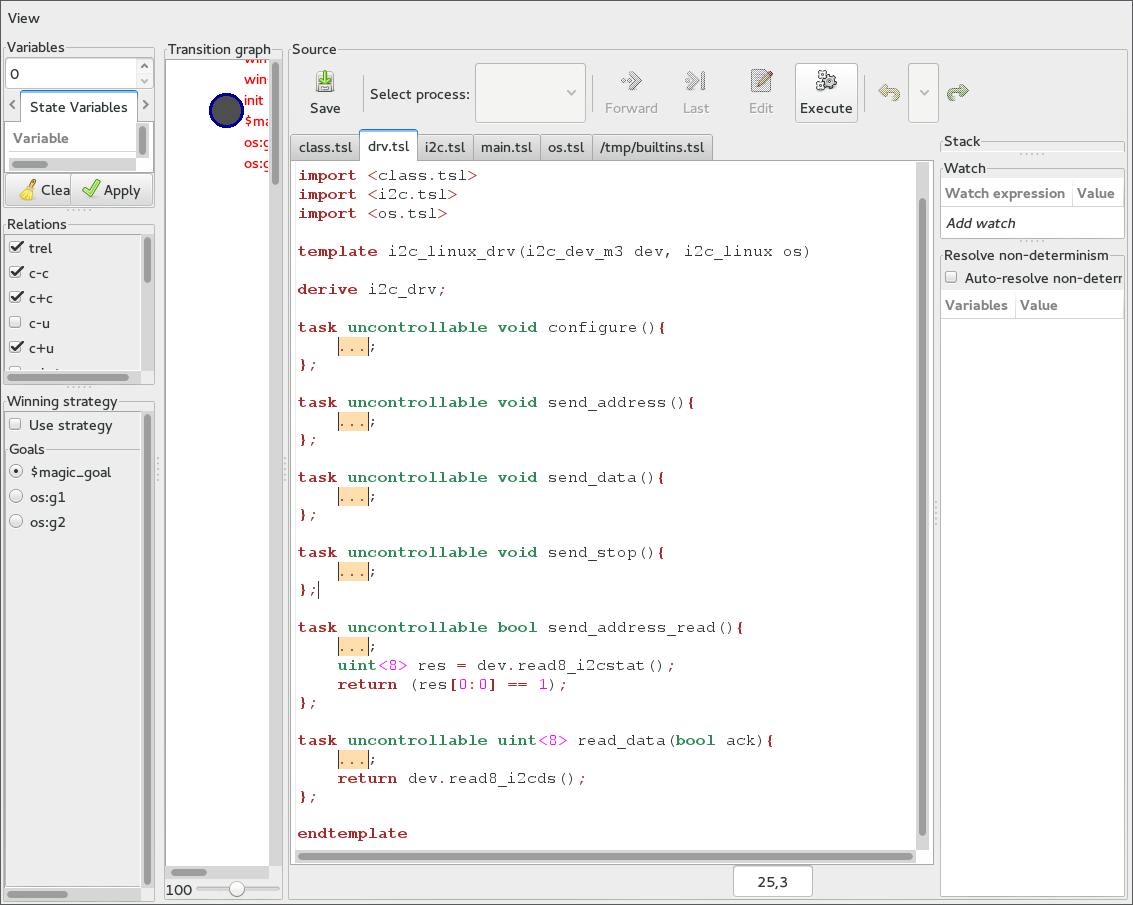
\includegraphics[width=\linewidth]{imgs/screenshot_1.png}
    \caption{Termite driver source code tab}
    \label{fig:driver_tab}
\end{figure}

\begin{figure}
    \center
    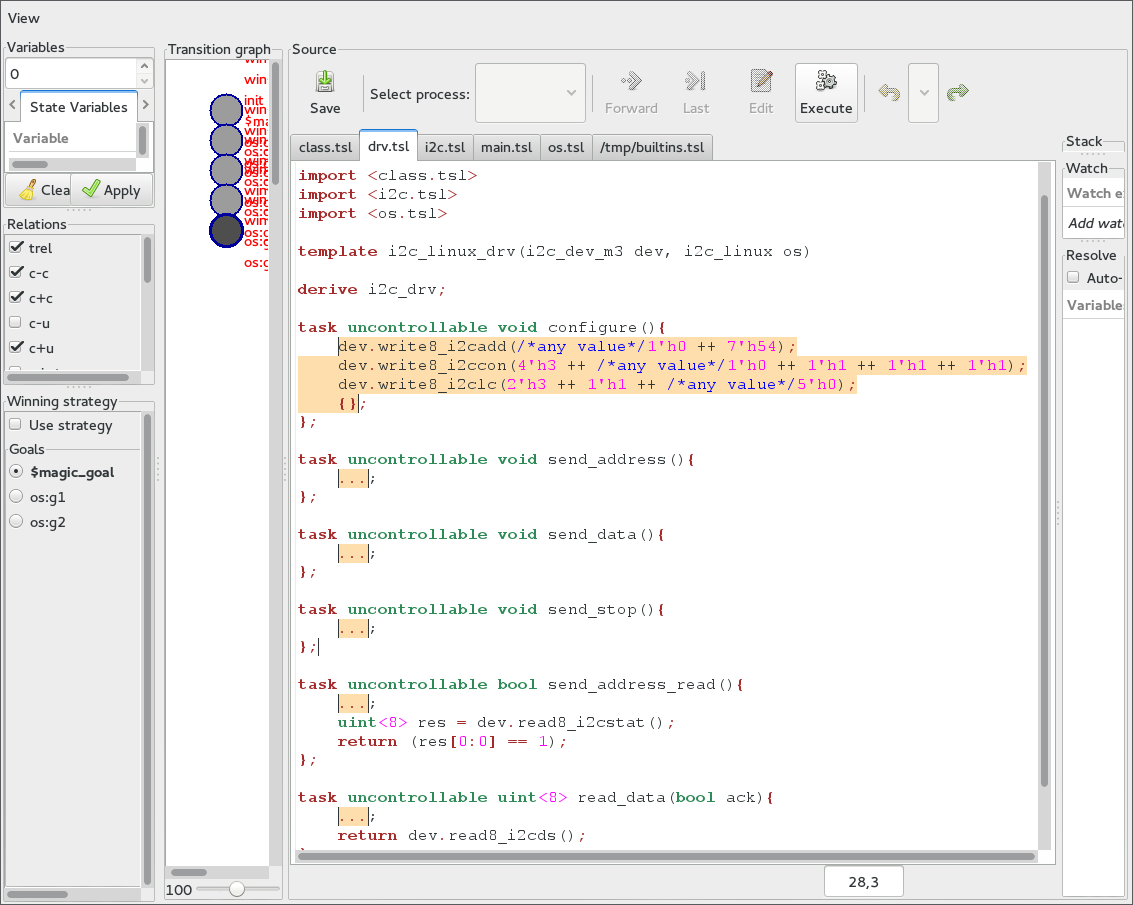
\includegraphics[width=\linewidth]{imgs/screenshot_2.png}
    \caption{Termite driver source code tab after code generation}
    \label{fig:driver_tab_gen}
\end{figure}

\section{Master write}
\label{a:sec_master_write}

We continue from where we left off in the \code{pos} process in the OS spec. We first set a flag to signal that initialisation was successful and then we enter a forever loop (Section~\ref{sec:loops}). On each iteration, the loop non-deterministically chooses between performing a master read or a master write transaction. For the sake of brevity we do not cover synthesis of the master read transaction. Assuming execution of the process enters the \code{master\_write} function we end up at line~\ref{l:os_master_write}.

This function models the behavior we expect of the \code{send\_address}, \code{send\_data} \code{send\_stop} sequence of driver functions. It uses a state variable \code{master\_state} to keep track of the current state of the master transmission. The code is a complex mess due to deficiencies of the specification language but it implements the state machine given in Figure~\ref{fig:master_sm}.

Note the two \emph{virtual callbacks} (similar to virtual functions) \code{address\_written} and \code{data\_sent} on lines~\ref{l:os_address_written} and~\ref{l:os_data_sent} respectively. They are invoked by the device state machine when the address writing and data sending phases complete. 

\lstinputlisting[style=tsl2]{i2c/i2c.tsl}
%
%\lstinputlisting[style=tsl2]{i2c/class.tsl}
%\lstinputlisting[style=tsl2]{i2c/drv.tsl.synthesized}
%\lstinputlisting[style=tsl2]{i2c/main.tsl}
